\documentclass{beamer}
\usepackage{amsmath,amsfonts,amssymb,amsthm,bm,extarrows,mathrsfs,dutchcal}
\usepackage{ctex}
\setCJKfamilyfont{kai}[AutoFakeBold]{simkai.ttf}
\newcommand*{\kai}{\CJKfamily{kai}}
\setCJKfamilyfont{song}[AutoFakeBold]{SimSun}
\newcommand*{\song}{\CJKfamily{song}}
\usepackage{tikz}
\usepackage{changepage}
\title[COVID_19 Analysis]{\textbf{COVID-19疫情数据的简要统计分析与预测}}
\subtitle{《MATLAB程序设计》大作业汇报}
\author[王逸扬,杨耕智]{王逸扬(19300180016)\and \\ 杨耕智(19300180112)}
\date{2022年5月30日}

\begin{document}
\frame{\titlepage}
\begin{frame}
\frametitle{目录}
    \begin{itemize}
        \item 数据导入、缺失值处理的类\texttt{StatisticsAnalysis};
        \item 长期性分析(自回归分析、周期性)
        \item 短期性分析(聚类分析、基于LSTM模型的预测分析)
    \end{itemize}
\end{frame}
\begin{frame}
\frametitle{数据导入、缺失值处理的类\texttt{StatisticsAnalysis}}
    参数:
    \begin{itemize}
        \item \texttt{\color{blue}TablePath}, \texttt{\color{blue}Table};
        \item \texttt{\color{blue}ImportOptions} 修改\texttt{detectImportOptions}中的参数;
        \item \texttt{\color{blue}SelectTableOptions} 检索表格;
        \item \texttt{\color{blue}MissingValuesOptions} 缺失值探测、处理;
        \item \texttt{\color{blue}TagsGenerateOptions} 计算并添加统计指标到\texttt{Table.Properties.CustomProperties}.
    \end{itemize}
\end{frame}
\begin{frame}
\frametitle{缺失值处理——「新增-累计」数据}
    \begin{minipage}{\textwidth}
        \centering
        \begin{tikzpicture}[scale=0.6]
            \draw (0,0) -- (1,0) -- (1,3) -- (0,3) -- (0,0);
            \draw (0,1) -- (2,1) -- (2,3) -- (1,3);
            \draw (0,2) -- (2,2);
            \coordinate [label=90:$I$] (I) at (0.5,3);
            \coordinate [label=90:$A$] (A) at (1.5,3);
            \coordinate [label=-90:$(P)$] (P) at (1,-3);
        \end{tikzpicture}
        \quad\quad
        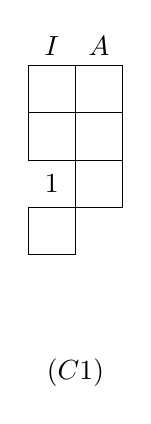
\begin{tikzpicture}[scale=0.6]
            \draw (0,0) -- (1,0) -- (1,3) -- (0,3) -- (0,1) -- (2,1) -- (2,3) -- (1,3);
            \draw (0,2) -- (2,2) -- (2,0) -- (1,0) -- (1,-1) -- (0,-1) -- (0,0);
            \coordinate [label=90:$1$] (P1) at (0.5,0.1);
            \coordinate [label=90:$I$] (I) at (0.5,3);
            \coordinate [label=90:$A$] (A) at (1.5,3);
            \coordinate [label=-90:$(C1)$] (C1) at (1,-3);
        \end{tikzpicture}
        \quad\quad
        \begin{tikzpicture}[scale=0.6]
            \draw (0,0) -- (1,0) -- (1,3) -- (0,3) -- (0,1) -- (2,1) -- (2,3) -- (1,3);
            \draw (0,2) -- (2,2) -- (2,0) -- (1,0) -- (1,-1) -- (0,-1) -- (0,0);
            \draw (2,0) -- (2,-1) -- (1,-1) -- (1,-2) -- (2,-2) -- (2,-1);
            \draw (1,-2) -- (0,-2) -- (0,-3) -- (1,-3) -- (1,-2);
            \coordinate [label=90:$1$] (P1) at (0.5,0.1);
            \coordinate [label=90:$2$] (P2) at (0.5,-1.9);
            \coordinate [label=90:$I$] (I) at (0.5,3);
            \coordinate [label=90:$A$] (A) at (1.5,3);
            \coordinate [label=-90:$(C2)$] (C2) at (1,-3);
            \coordinate [label=0:$\cdots\cdots$] (CD) at (2.5,0.25);
        \end{tikzpicture}
    \end{minipage}
    \begin{itemize}
        \item {\color{blue}需要插值的$P$、$C$两种情况的处理}:默认线性插值,也可以传入自定义的插值函数句柄,例如\texttt{spline};
        \item {\color{blue}增量数据不单调的处理}: 不处理/衰减地分配到前几日/传入函数句柄处理.
    \end{itemize}
\end{frame}
\begin{frame}
\frametitle{长期性分析}
    自回归函数\texttt{autocorr}、偏自回归函数\texttt{parcorr}、周期性.
    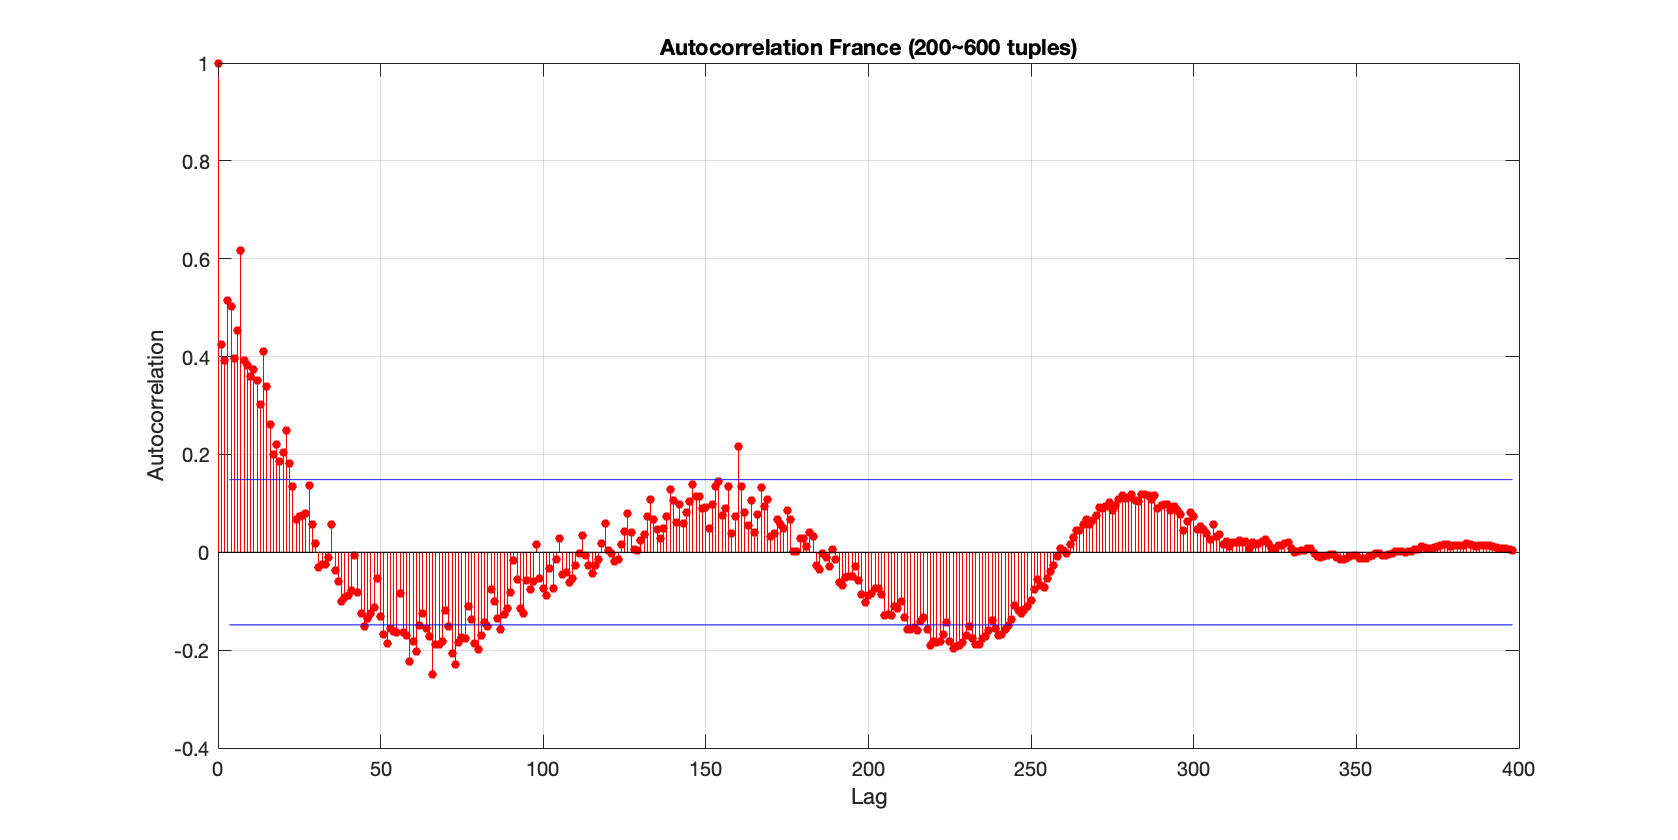
\includegraphics[width=\textwidth]{./images/France_ACF.png}
\end{frame}
\begin{frame}
\frametitle{短期性分析(地区数据的$k$-mean聚类)}
    主成分分析. 肘部原理$\Rightarrow k=4$.
    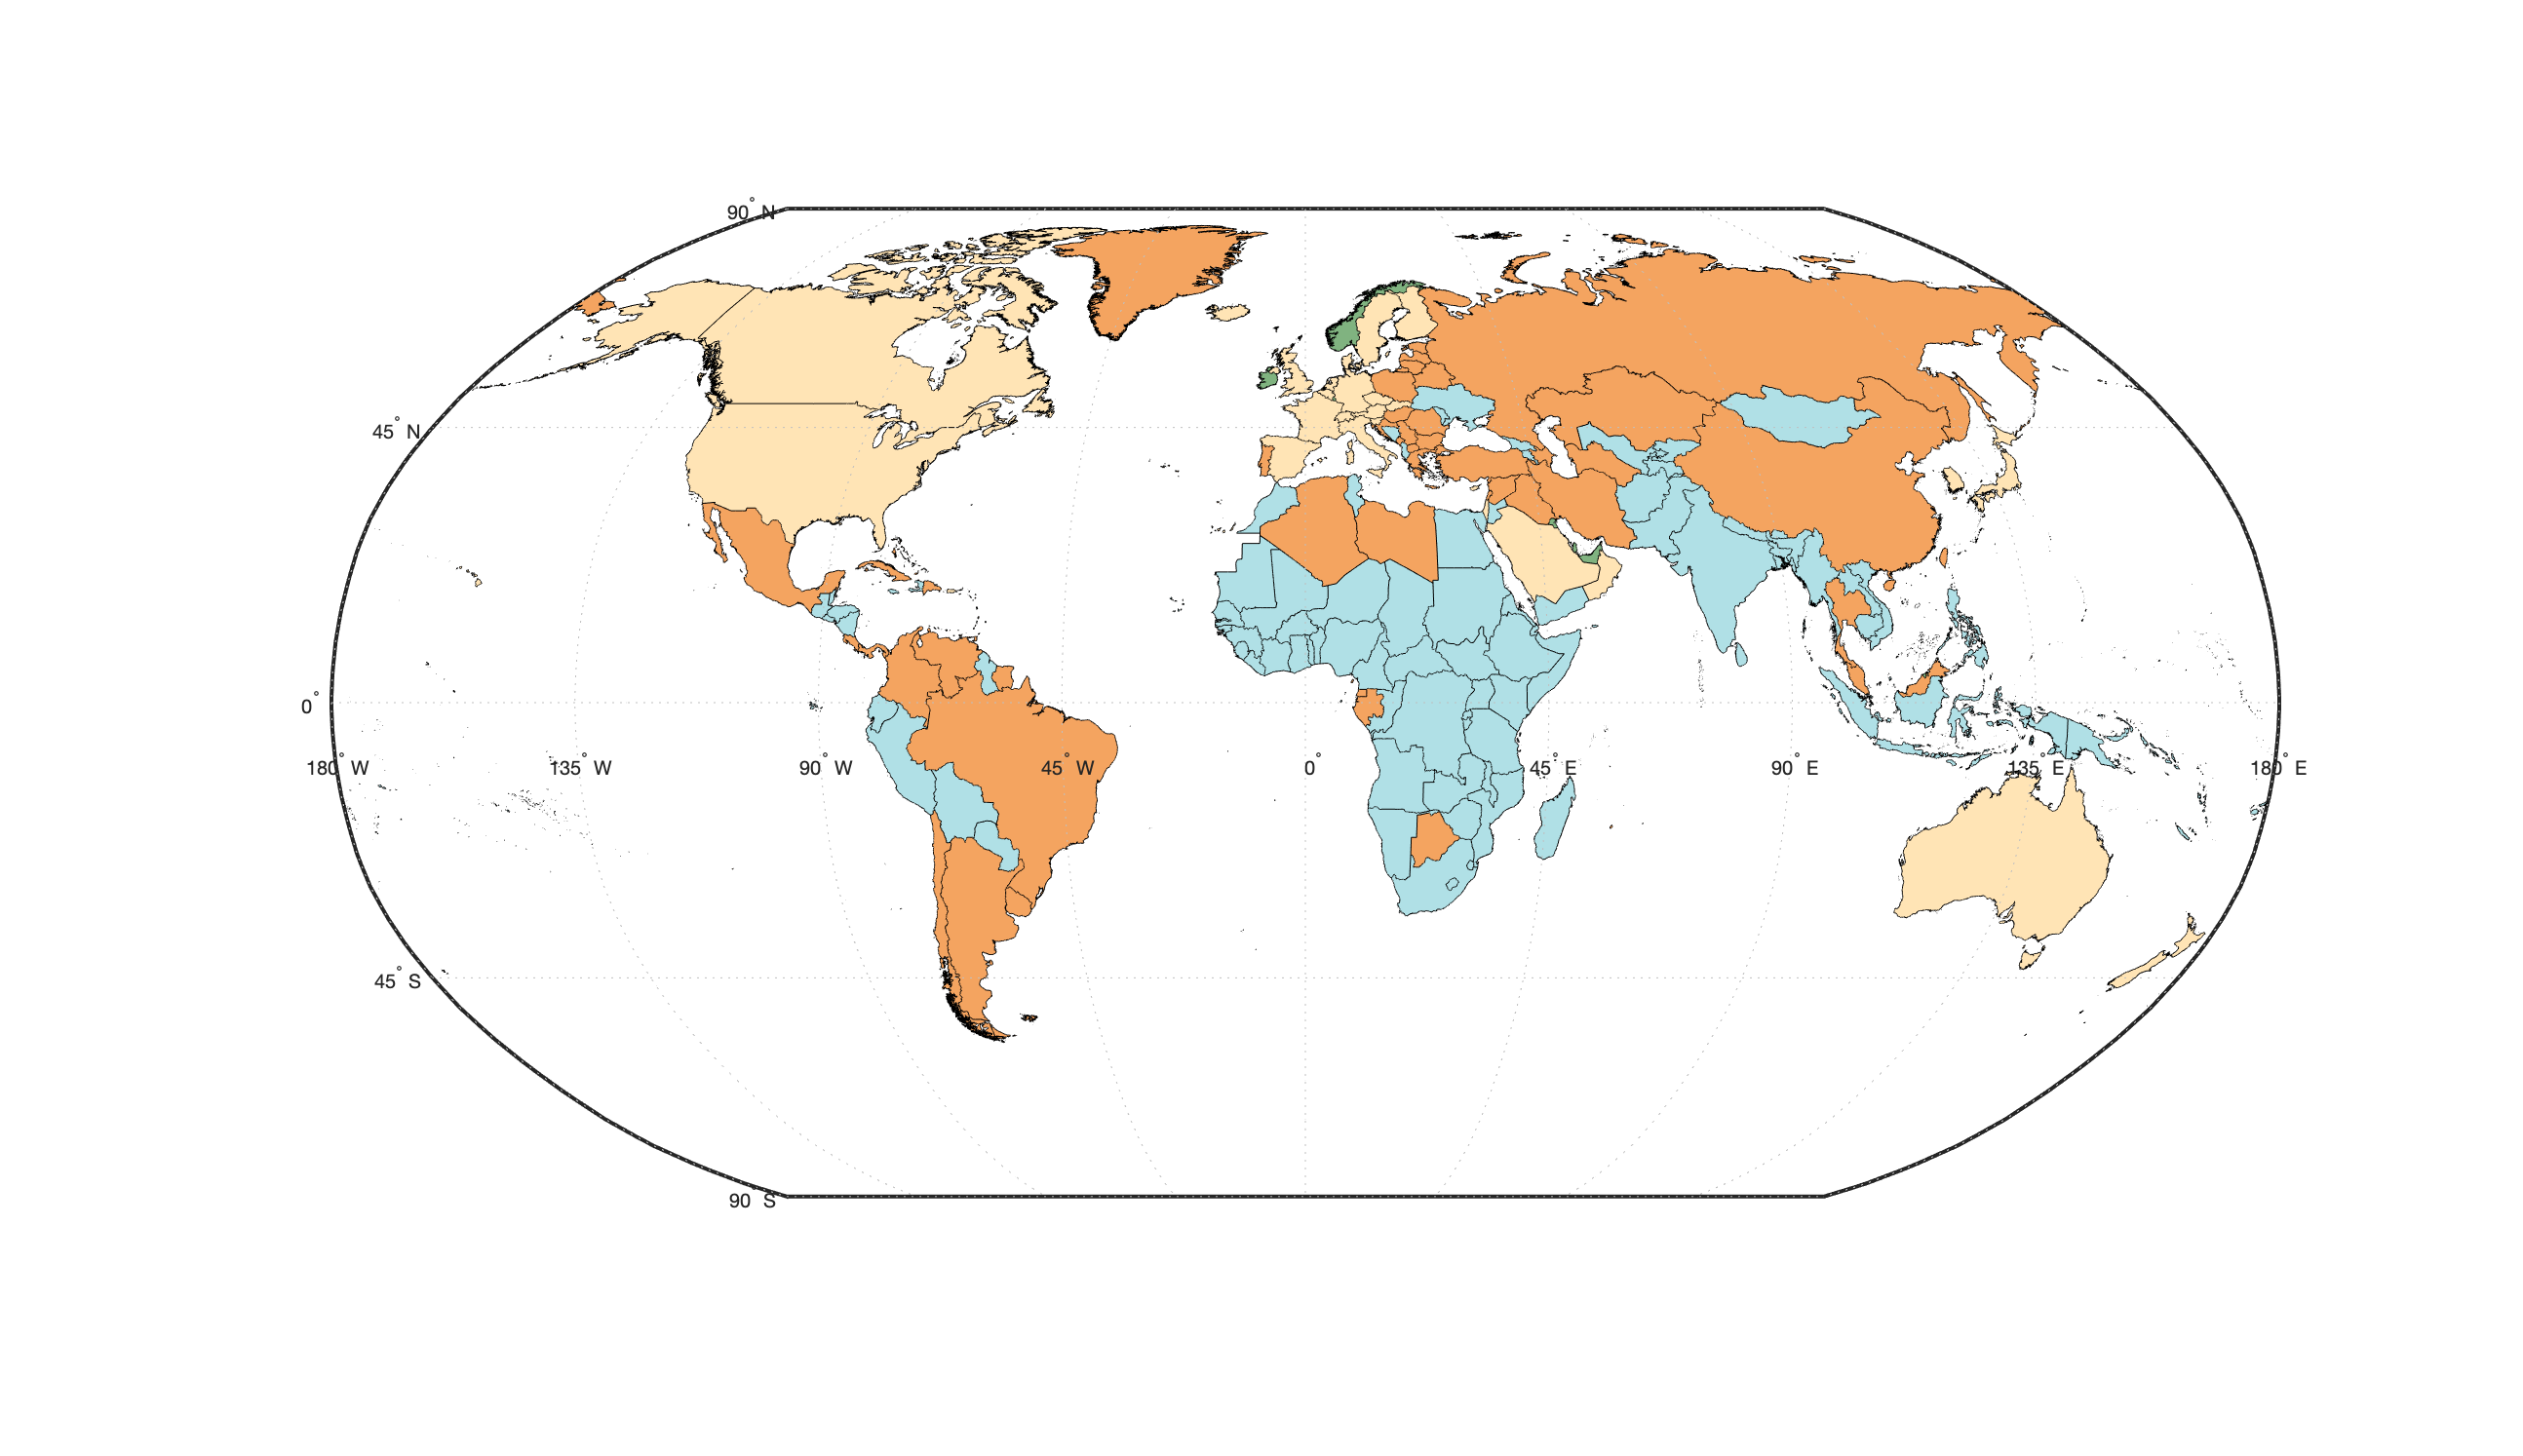
\includegraphics[width=\textwidth]{./images/World_Classification.png}
\end{frame}
\begin{frame}
\frametitle{短期性分析(时间序列特征的谱系聚类)}
    某时期各国家的:(峰峰值、平均值、标准差)/人口,偏度和峰度.
    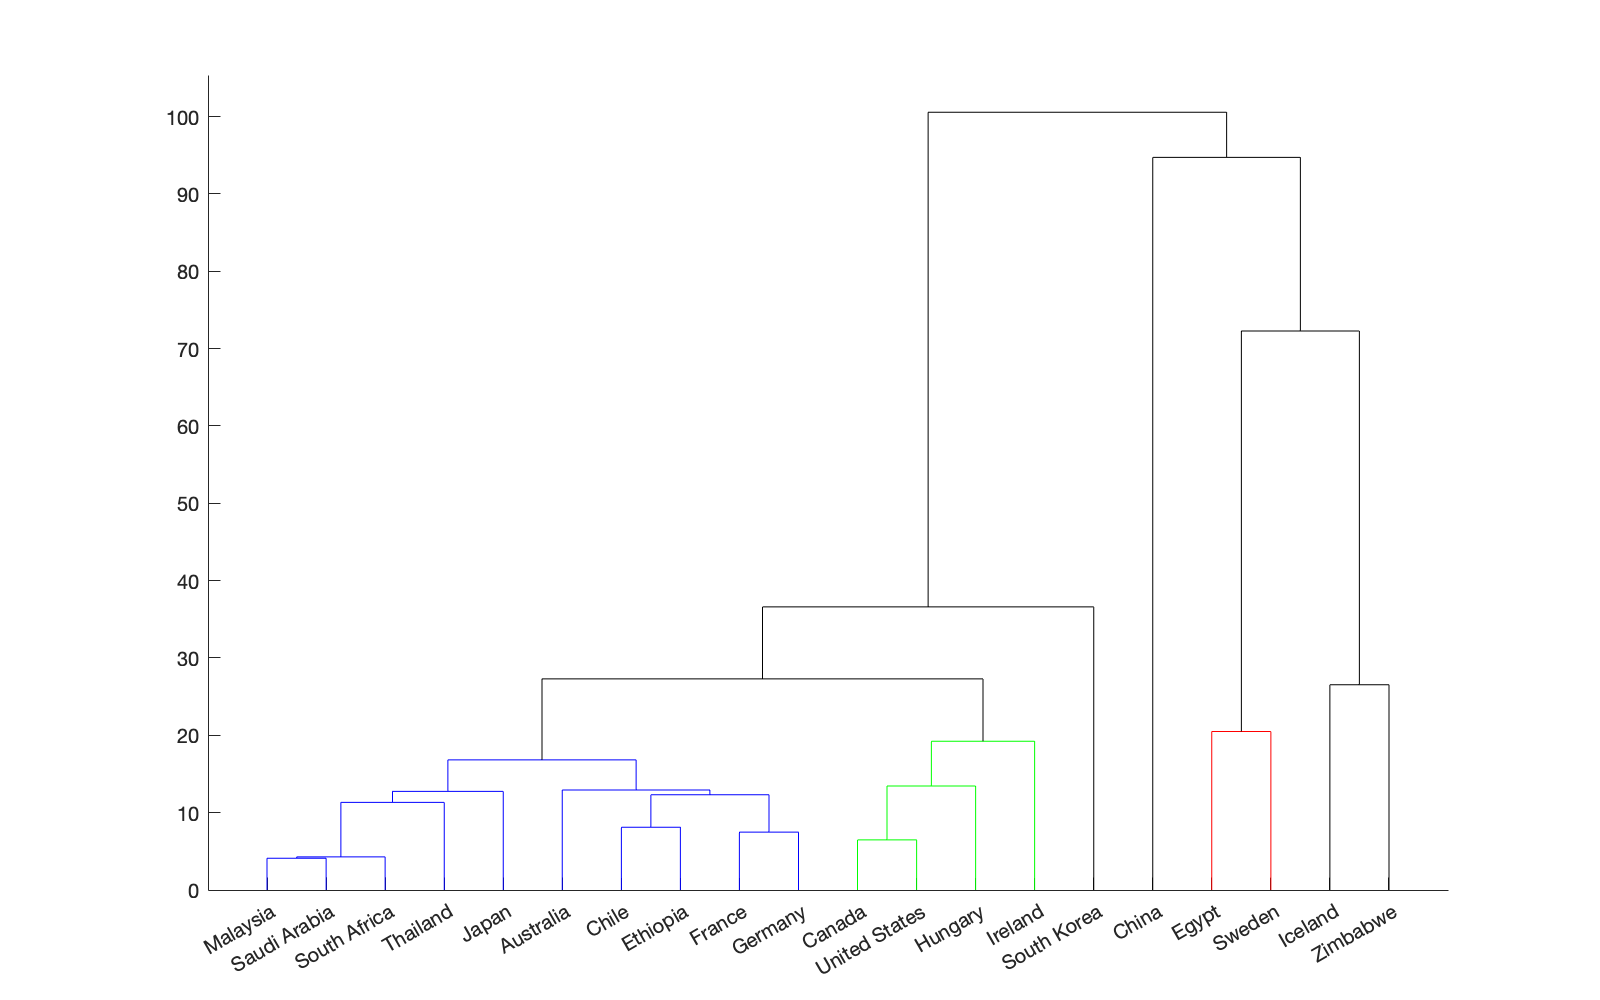
\includegraphics[width=\textwidth]{./images/Tree_2.png}
\end{frame}
\begin{frame}
\frametitle{短期性分析(基于LSTM模型的预测分析)}
    MATLAB的神经网络工具箱. 简单情形$\Rightarrow$ LSTM. 
    \begin{align*}
		&\texttt{sequenceInputLayer(8)} \\
        \rightarrow\quad&\texttt{fullyConnectedLayer(30)}\\
    	\rightarrow\quad&\texttt{reluLayer}\\
    	\rightarrow\quad&\texttt{lstmLayer(400)}\\
    	\rightarrow\quad&\texttt{reluLayer}\\
    	\rightarrow\quad&\texttt{fullyConnectedLayer(30)}\\
    	\rightarrow\quad&\texttt{reluLayer}\\
    	\rightarrow\quad&\texttt{fullyConnectedLayer(numResponses)}\\
    	\rightarrow\quad&\texttt{regressionLayer}
	\end{align*}
\end{frame}
\begin{frame}
\frametitle{短期性分析(基于LSTM模型的预测分析)}
    \begin{adjustwidth}{-1.5cm}{}
        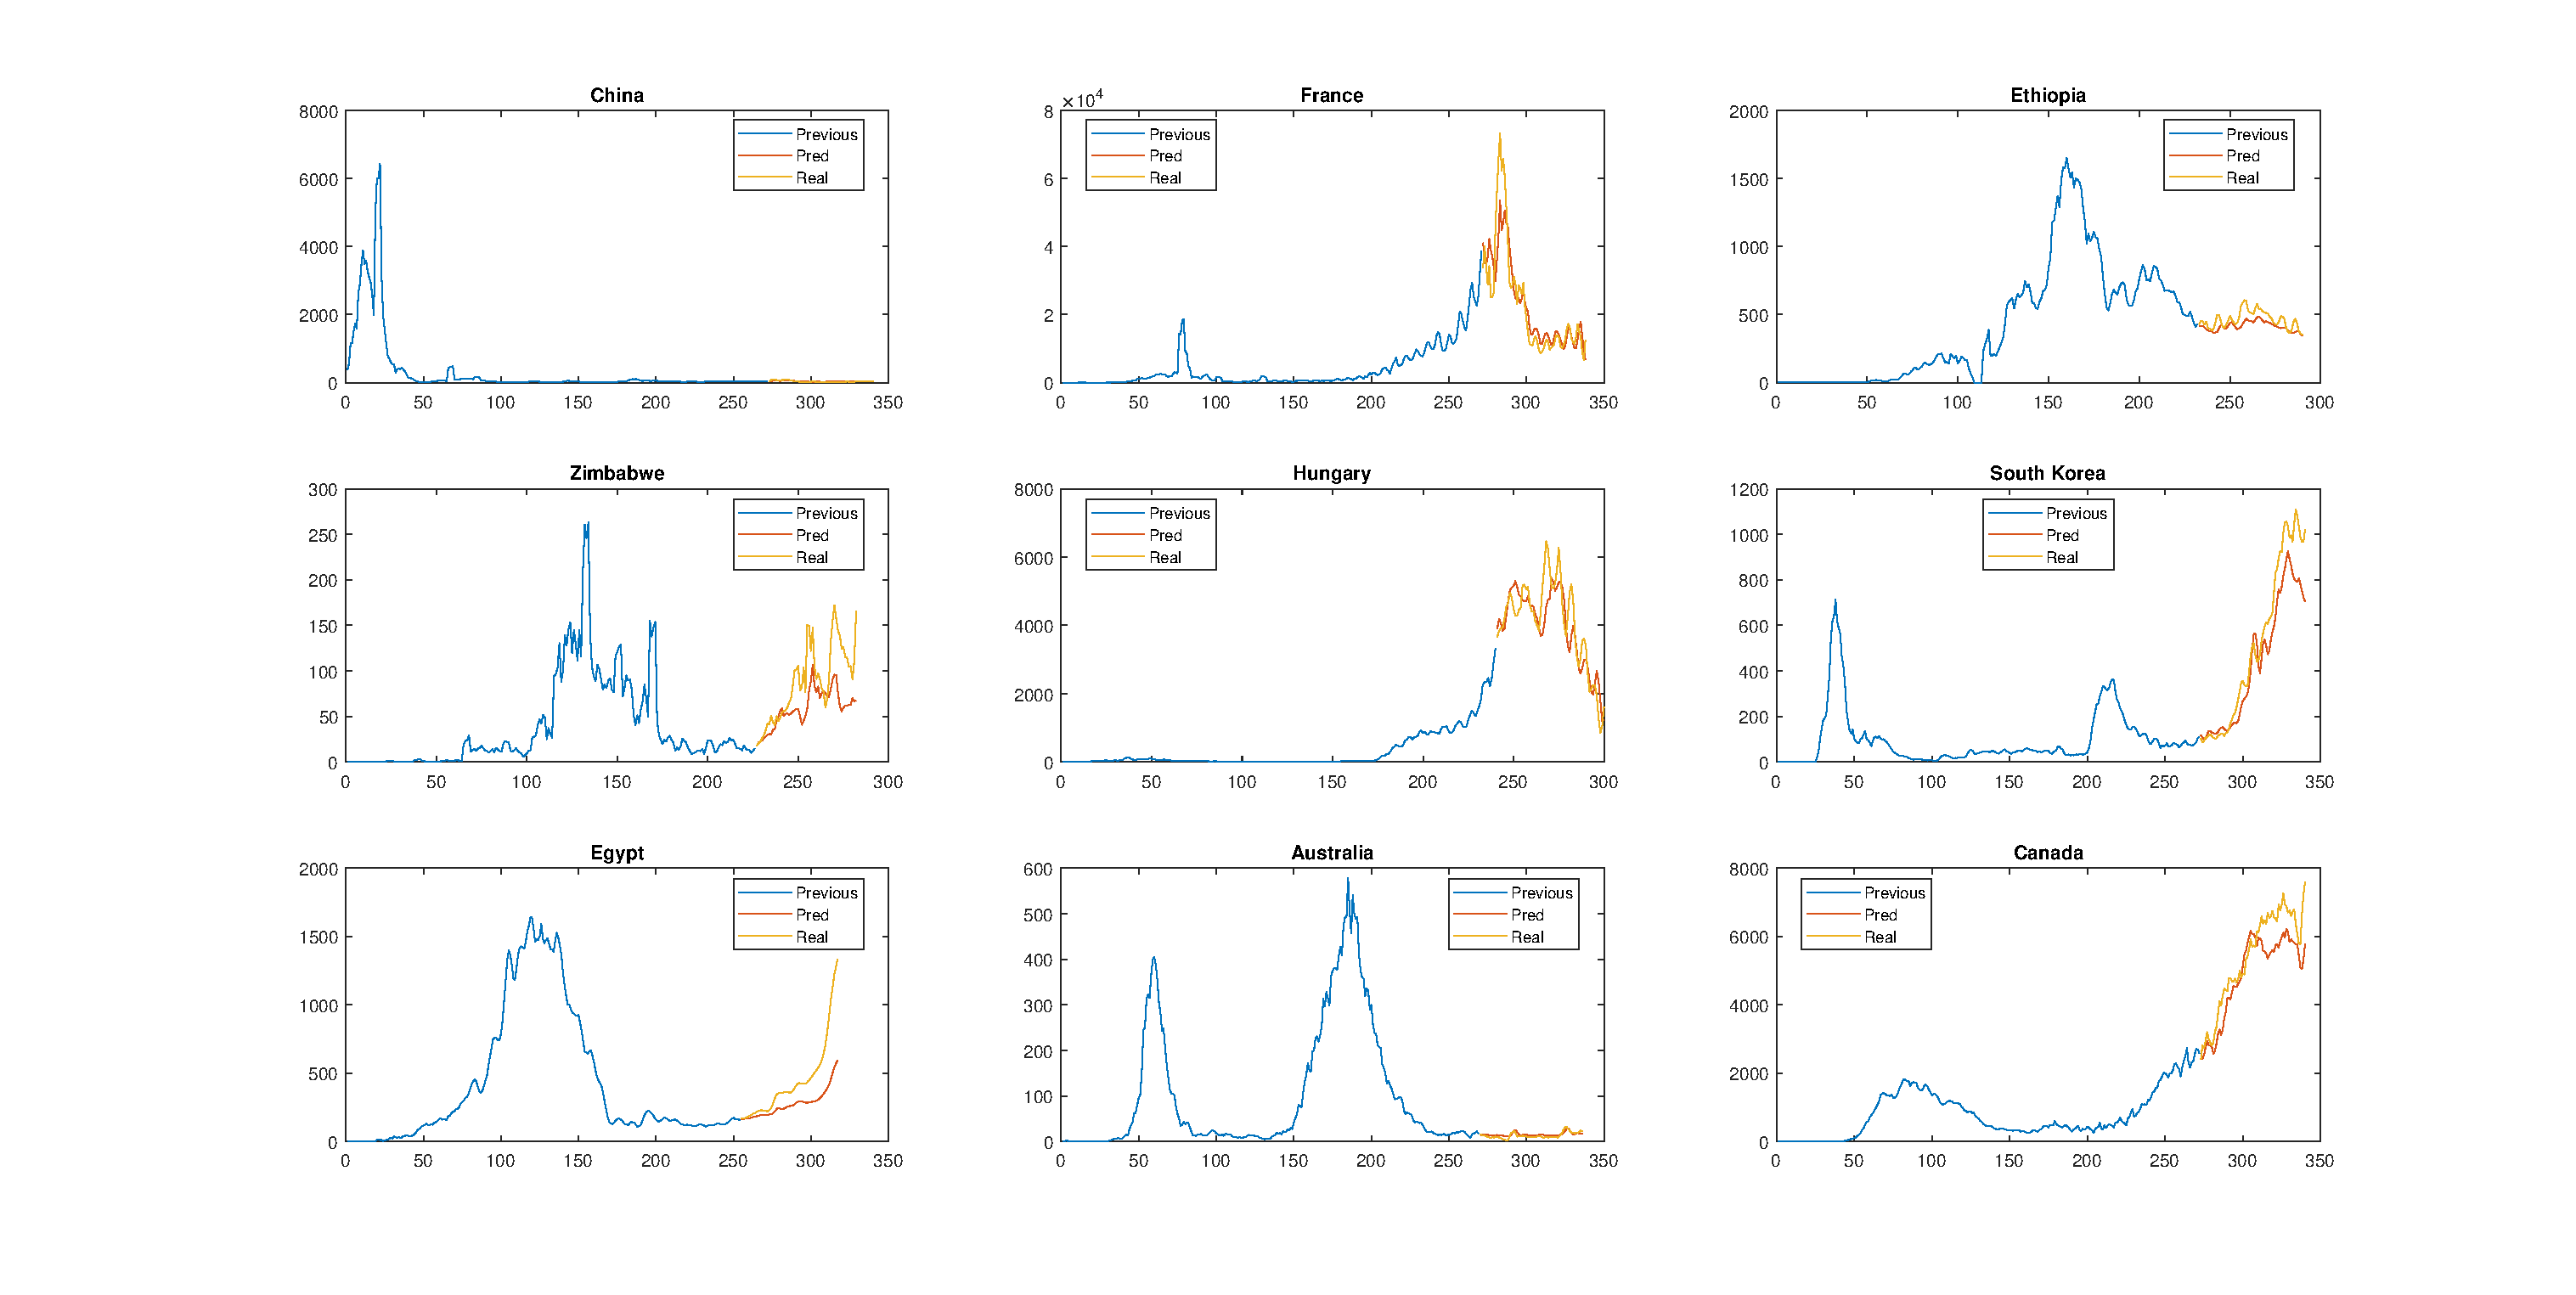
\includegraphics[height=8cm, width=14cm]{./images/Chapter5/Pred.eps}
    \end{adjustwidth}
\end{frame}
\begin{frame}
    \begin{center}
    以上就是我们对COVID-19数据集的分析,\\
    水平有限,多有疏漏,恳请各位批评指正. \\
    \quad\\
    最后,感谢陈阳老师和两位助教一学期以来的教导与帮助!
    \end{center}
\end{frame}
\end{document}